\documentclass[11pt]{article}
%%%%%%%%%%%%%%%%%%%%%%%%%%%%%%%%%%%%%%%%%%%%%%%%%%%%%%%%%%%%%%%%%%%%%%%
\usepackage{amsfonts,amssymb,amsthm,amsmath}
\usepackage{enumerate}
\usepackage[flushleft]{threeparttable}
\usepackage[format=hang,font=normalsize,labelfont=bf]{caption}
\usepackage{amsmath}
\usepackage{datetime}
\usepackage{array}
\usepackage{multirow}
\usepackage{delarray}
\usepackage{eurosym}
\usepackage{amssymb}
\usepackage{amsthm}
\usepackage{natbib}
\usepackage{setspace}
\usepackage[colorlinks=true,urlcolor=cmu,citecolor=cmu,linkcolor=cmu]{hyperref}
\usepackage{float,color}
\usepackage[pdftex]{graphicx}
\usepackage{lscape}
\usepackage{pdflscape}
% \usepackage{geometry}
\usepackage{subfig}
\usepackage{epsf}
\usepackage{multicol}
\usepackage{bbm}
\usepackage{epstopdf}
\usepackage{lscape}
\usepackage{bibentry}
\usepackage[font={bf}]{caption}
\usepackage{booktabs}

\newcommand{\argmin}{\operatornamewithlimits{argmin}}
\newcommand{\argmax}{\operatornamewithlimits{argmax}}
\newcommand*\diff{\mathop{}\!\mathrm{d}}

\listfiles
\makeatletter
\renewcommand\BR@b@bibitem[2][]{\BR@bibitem[#1]{#2}\BR@c@bibitem{#2}} 
\makeatother

\usepackage{color}
\definecolor{cmu}{rgb}{0.76,0,0}

\usepackage{algorithm2e}


\usepackage{geometry}
\geometry{verbose,tmargin=0.75in,bmargin=1in,lmargin=0.75in,rmargin=0.75in,headheight=0.25in}


\usepackage[section]{placeins}
\hypersetup{colorlinks,linkcolor=blue,urlcolor=blue,citecolor=blue}
\theoremstyle{definition}
\newtheorem{theorem}{Theorem}
\newtheorem{acknowledgement}[theorem]{Acknowledgement}
%\newtheorem{algorithm}[theorem]{Algorithm}
\newtheorem{axiom}[theorem]{Axiom}
\newtheorem{case}[theorem]{Case}
\newtheorem{claim}[theorem]{Claim}
\newtheorem{conclusion}[theorem]{Conclusion}
\newtheorem{condition}[theorem]{Condition}
\newtheorem{conjecture}[theorem]{Conjecture}
\newtheorem{corollary}[theorem]{Corollary}
\newtheorem{criterion}[theorem]{Criterion}
\newtheorem{definition}{Definition} % Number definitions on their own
\newtheorem{derivation}{Derivation} % Number derivations on their own
\newtheorem{example}[theorem]{Example}
\newtheorem{exercise}[theorem]{Exercise}
\newtheorem{lemma}[theorem]{Lemma}
\newtheorem{notation}[theorem]{Notation}
\newtheorem{problem}[theorem]{Problem}
\newtheorem{proposition}{Proposition} % Number propositions on their own
\newtheorem{remark}[theorem]{Remark}
\newtheorem{solution}[theorem]{Solution}
\newtheorem{summary}[theorem]{Summary}
\numberwithin{equation}{section}

\newcommand{\R}{\mathbb{R}}

\linespread{1.3}
\begin{document}

\title{A Political Districting Algorithm with Communities of Interest\\
Online Appendix }
\author{Ryan Murray\thanks{Department of Mathematics,
Penn State University; email: rwm22@psu.edu.} \\
Penn State University  \\
\and Benjamin Tengelsen \thanks{Tepper School of Business, 
Carnegie Mellon University; email: btengels@cmu.edu.} \\
Carnegie Mellon University }
\maketitle


\begin{abstract}
This work proposes a new algorithm for drawing district boundaries. The algorithm is an adaptation of previous methods which minimize transport distances between constituents and representatives. The crucial adaptation is a modification in the distance which permits the algorithm to respect communities of interest. The problem is also rendered computationally tractable by some very recent regularizing methods. Finally, the results of the algorithm, along with the accompanying political ramifications, are presented for congressional districts across a large number of states.
\end{abstract}

\newpage{} \onehalfspacing
\tableofcontents

\newpage
\section{Data Desription }


\newpage
\section{National Results }



\newpage
\section{State by State Results }
\subsection{Alabama}
\begin{figure}[htb!] \centering
\caption{ Current Districts }
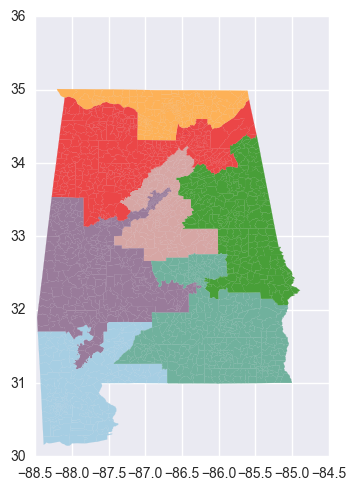
\includegraphics[width=5in,height=3in,keepaspectratio]{../maps/AL/static/before.png}
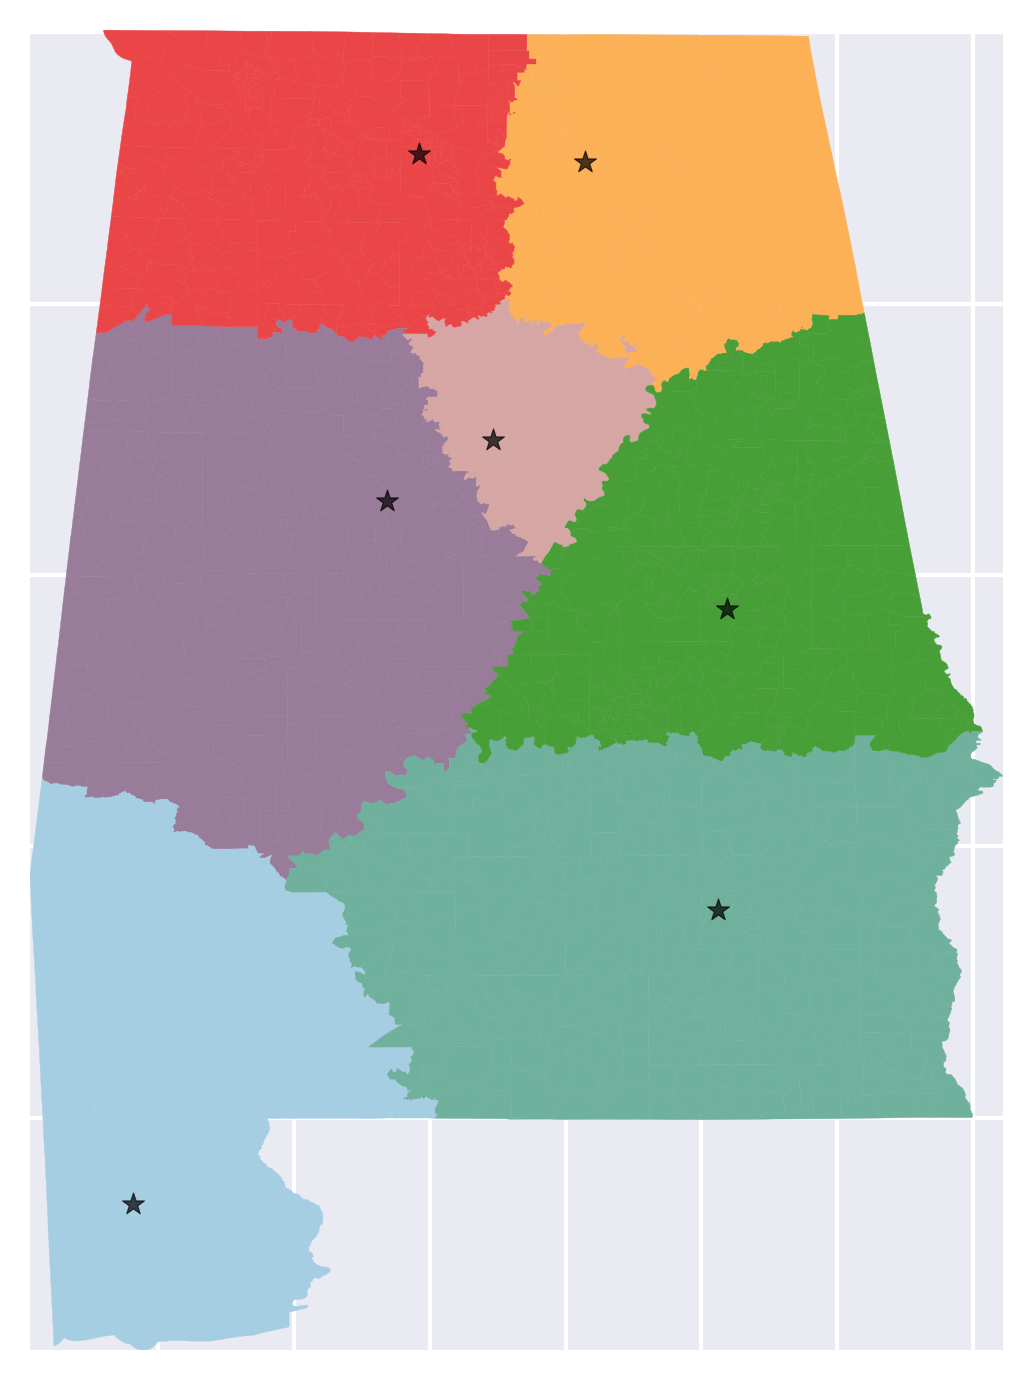
\includegraphics[width=5in,height=3in,keepaspectratio]{../maps/AL/static/0_0_after.png}
\caption{ New Districts ($\alpha_w$ = 1) }
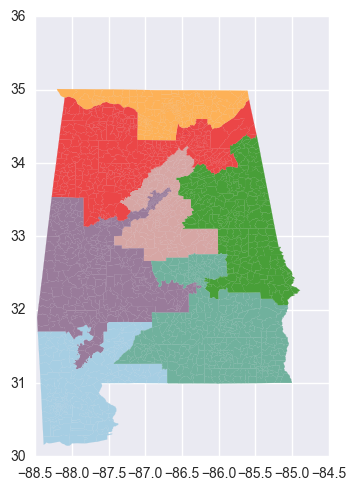
\includegraphics[width=5in,height=3in,keepaspectratio]{../maps/AL/static/before.png}
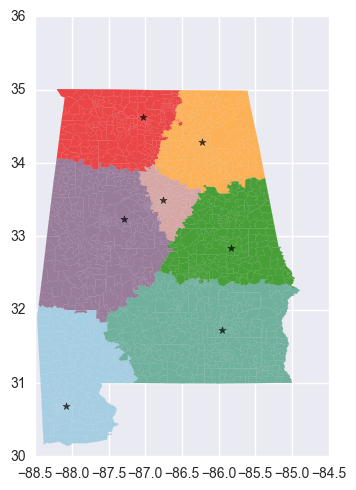
\includegraphics[width=5in,height=3in,keepaspectratio]{../maps/AL/static/0_25_after.png}
\end{figure}

\clearpage
\newpage

\begin{figure}[htb!] \centering
\caption{ Politics: democratic population (placeholder)}
\includegraphics[width=6in]{../analysis/AL/R_pct_kde.pdf}
\caption{ Demographics: black population }
\includegraphics[width=6in]{../analysis/AL/black_pct_kde.pdf}
\caption{ Demographics: hispanic population }
\includegraphics[width=6in]{../analysis/AL/hisp_pct_kde.pdf}
\end{figure}

\clearpage
\newpage

\begin{figure}[htb!] \centering
\caption{ Politics: democratic population (placeholder)}
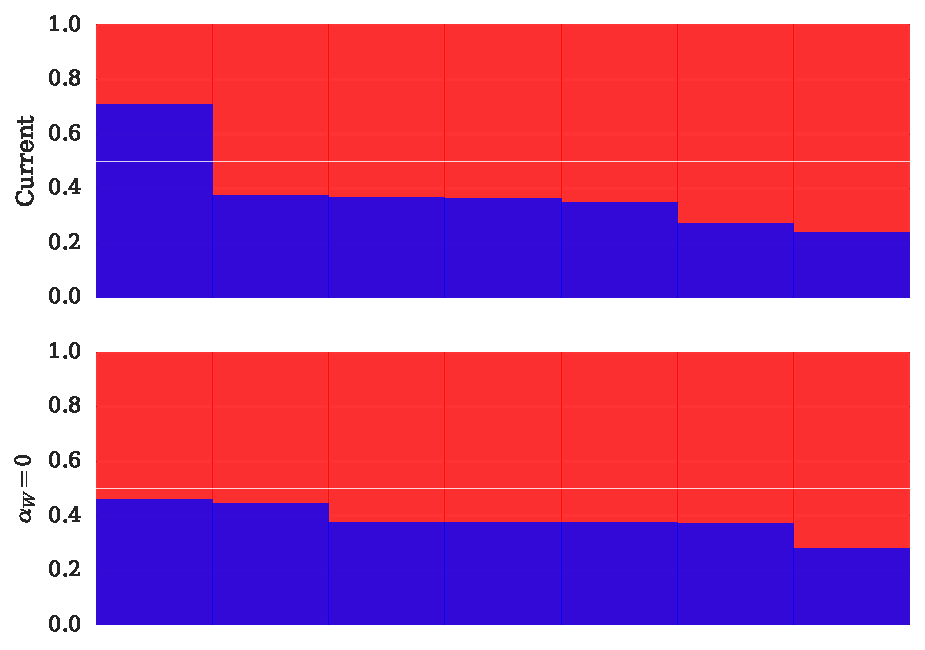
\includegraphics[width=6in]{../analysis/AL/barplot.pdf}
\end{figure}

\clearpage
\newpage

\subsection{Arkansas}
\begin{figure}[htb!] \centering
\caption{ Current Districts }
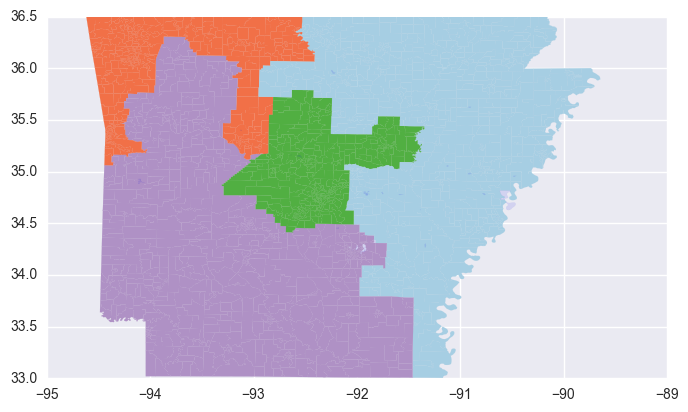
\includegraphics[width=4in,height=3in,keepaspectratio]{../maps/AR/static/before.png}
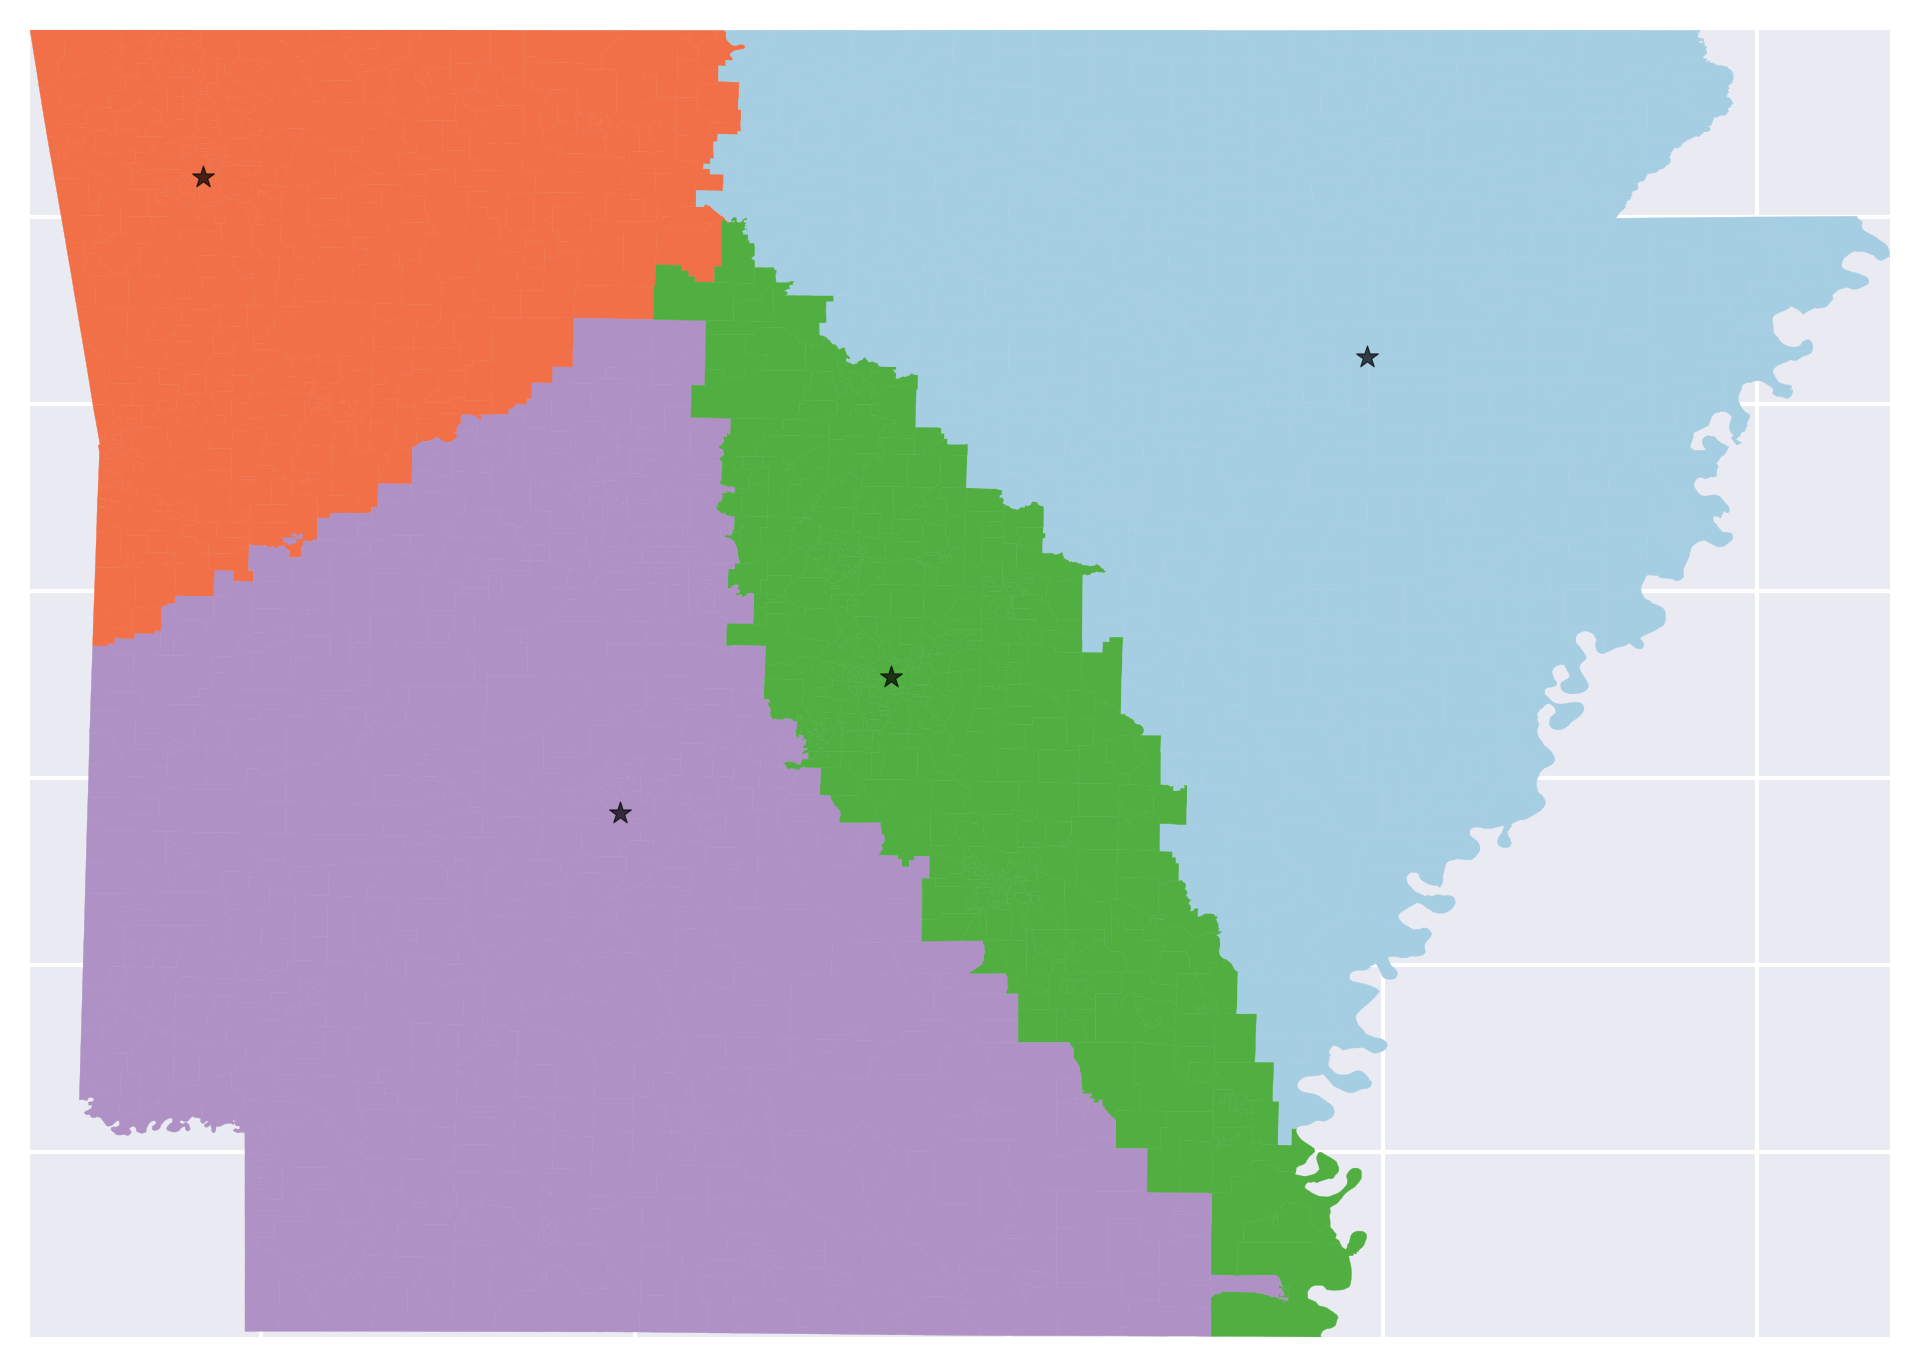
\includegraphics[width=4in,height=3in,keepaspectratio]{../maps/AR/static/0_0_after.png}
\caption{ New Districts ($\alpha_w$ = 1) }
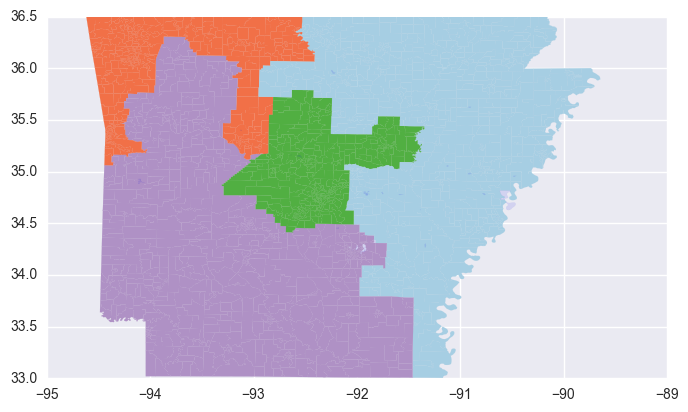
\includegraphics[width=4in,height=3in,keepaspectratio]{../maps/AR/static/before.png}
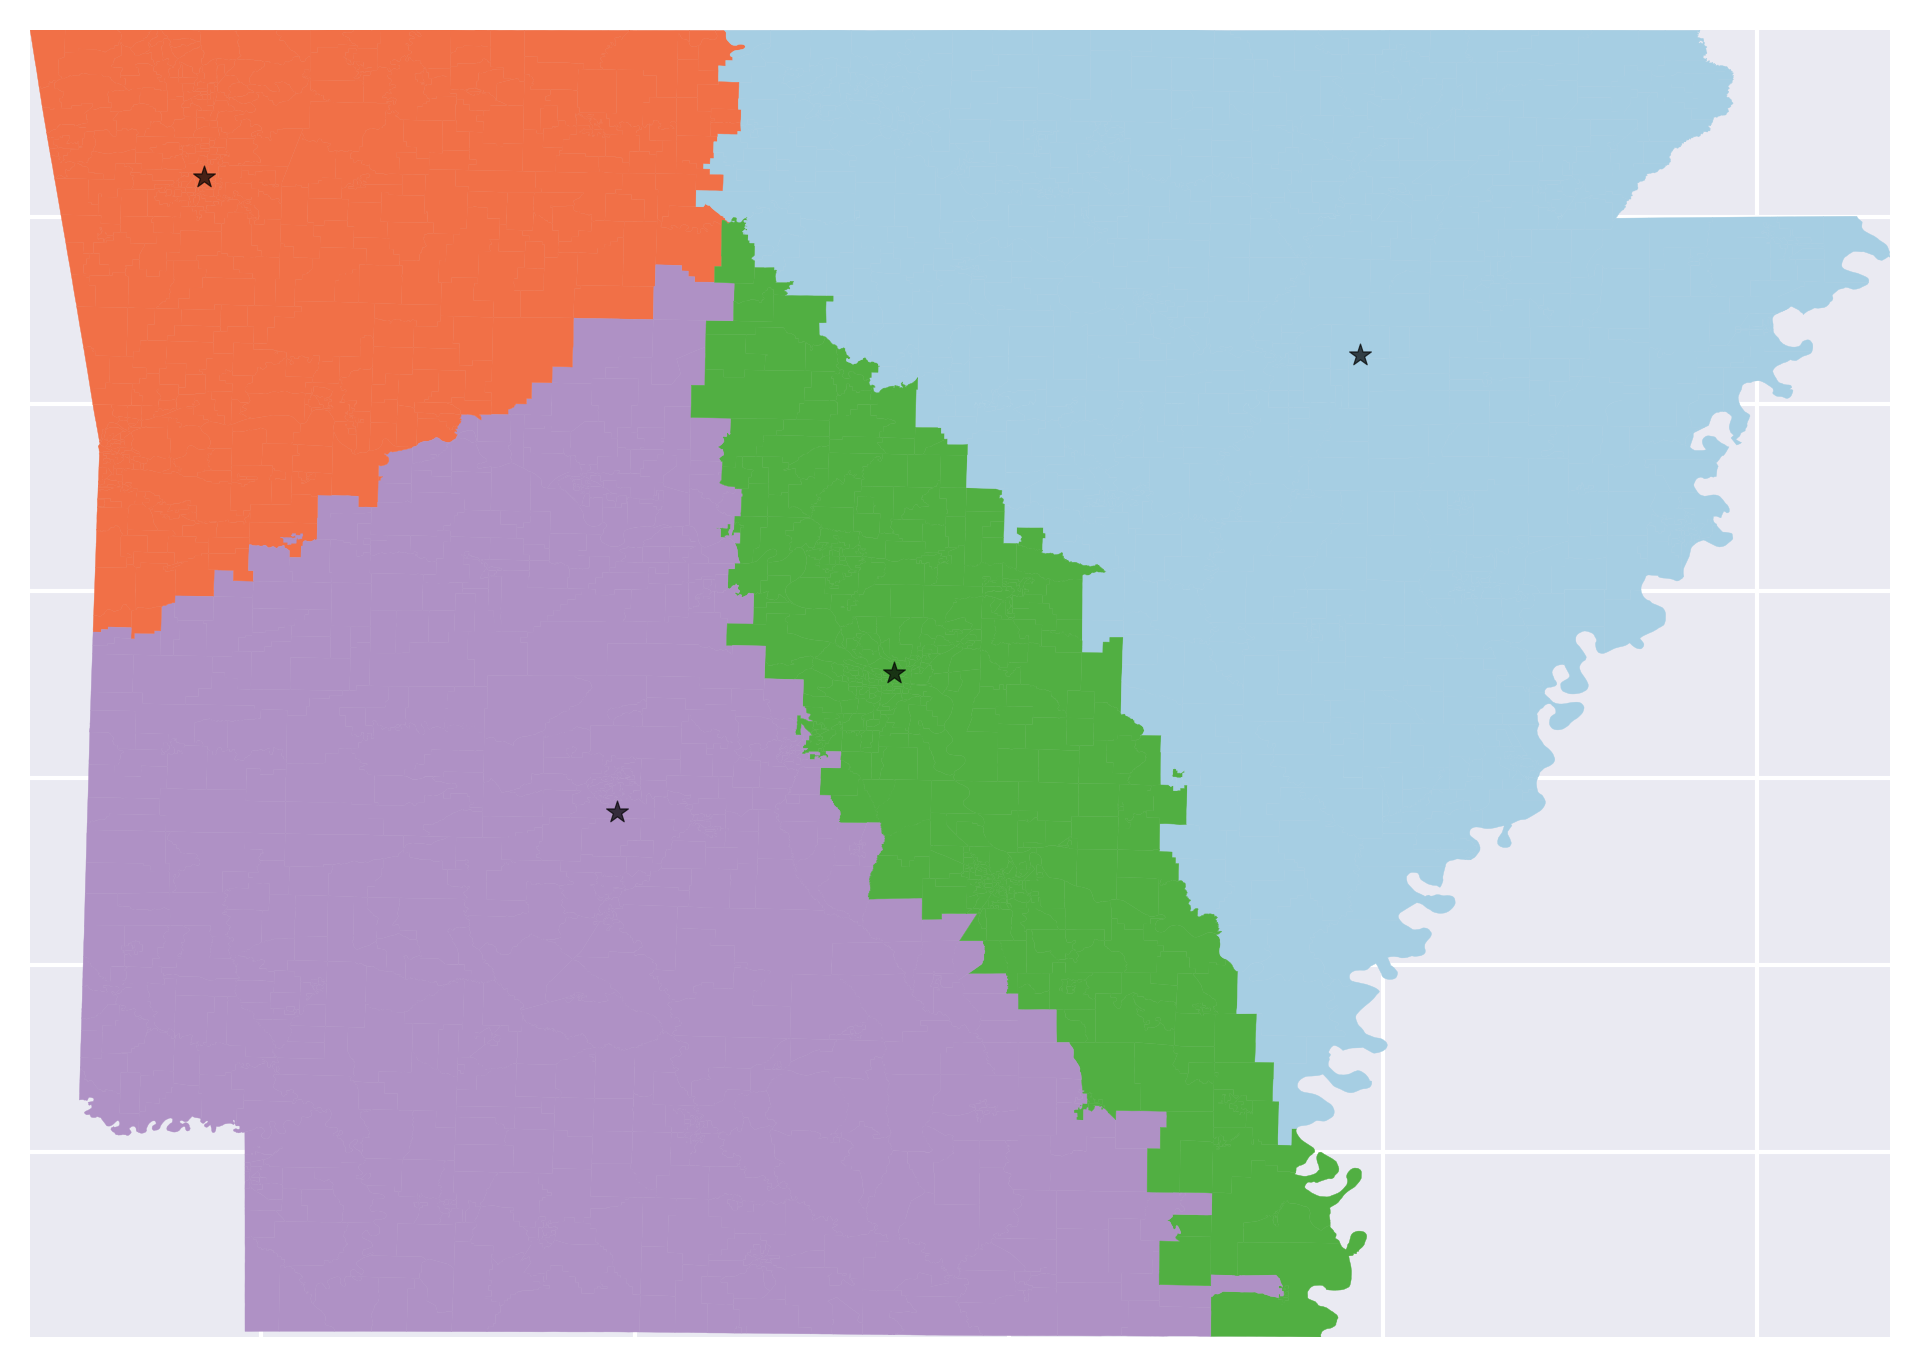
\includegraphics[width=4in,height=3in,keepaspectratio]{../maps/AR/static/0_25_after.png}
\end{figure}

\clearpage
\newpage

\begin{figure}[htb!] \centering
\caption{ Politics: democratic population (placeholder)}
\includegraphics[width=6in]{../analysis/AR/R_pct_kde.pdf}
\caption{ Demographics: black population }
\includegraphics[width=6in]{../analysis/AR/black_pct_kde.pdf}
\caption{ Demographics: hispanic population }
\includegraphics[width=6in]{../analysis/AR/hisp_pct_kde.pdf}
\end{figure}

\clearpage
\newpage

\begin{figure}[htb!] \centering
\caption{ Politics: democratic population (placeholder)}
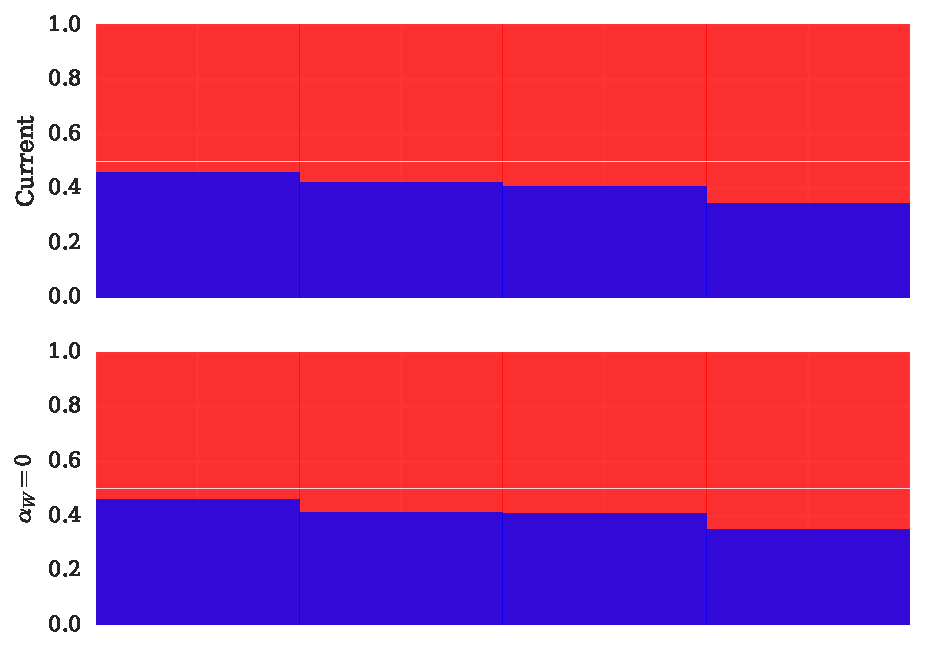
\includegraphics[width=6in]{../analysis/AR/barplot.pdf}
\end{figure}

\clearpage
\newpage

\subsection{Arizona}
\begin{figure}[htb!] \centering
\caption{ Current Districts }
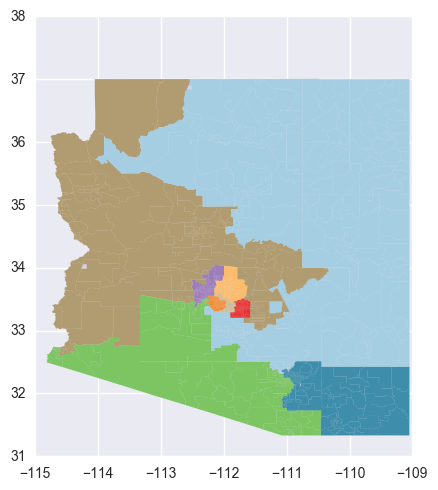
\includegraphics[width=5in,height=3in,keepaspectratio]{../maps/AZ/static/before.png}
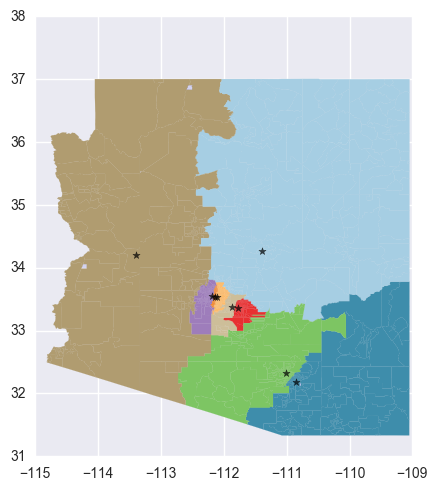
\includegraphics[width=5in,height=3in,keepaspectratio]{../maps/AZ/static/0_0_after.png}
\caption{ New Districts ($\alpha_w$ = 1) }
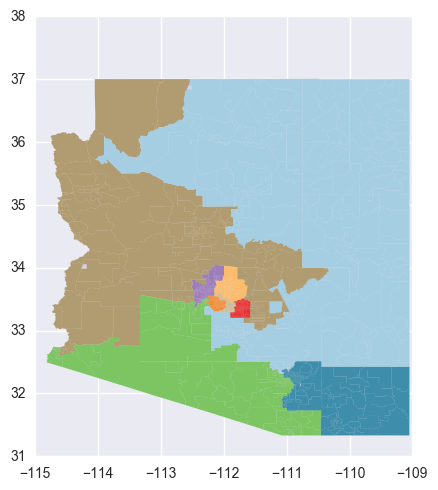
\includegraphics[width=5in,height=3in,keepaspectratio]{../maps/AZ/static/before.png}
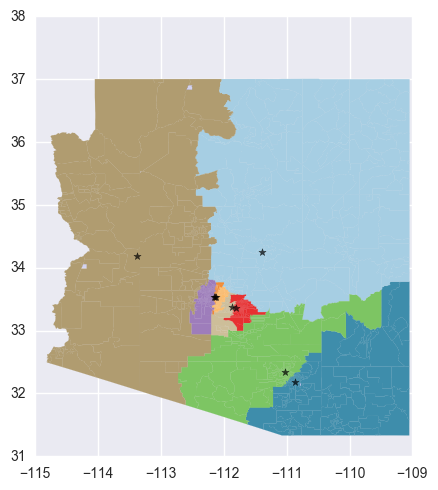
\includegraphics[width=5in,height=3in,keepaspectratio]{../maps/AZ/static/0_25_after.png}
\end{figure}

\clearpage
\newpage

\begin{figure}[htb!] \centering
\caption{ Politics: democratic population (placeholder)}
\includegraphics[width=6in]{../analysis/AZ/R_pct_kde.pdf}
\caption{ Demographics: black population }
\includegraphics[width=6in]{../analysis/AZ/black_pct_kde.pdf}
\caption{ Demographics: hispanic population }
\includegraphics[width=6in]{../analysis/AZ/hisp_pct_kde.pdf}
\end{figure}

\clearpage
\newpage

\begin{figure}[htb!] \centering
\caption{ Politics: democratic population (placeholder)}
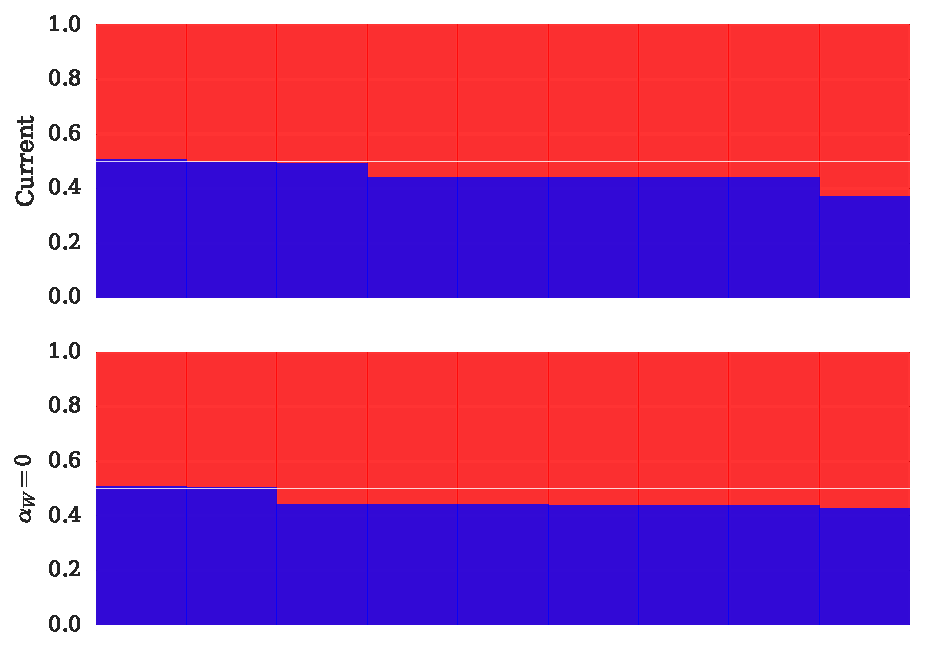
\includegraphics[width=6in]{../analysis/AZ/barplot.pdf}
\end{figure}

\clearpage
\newpage

\subsection{California}
\begin{figure}[htb!] \centering
\caption{ Current Districts }
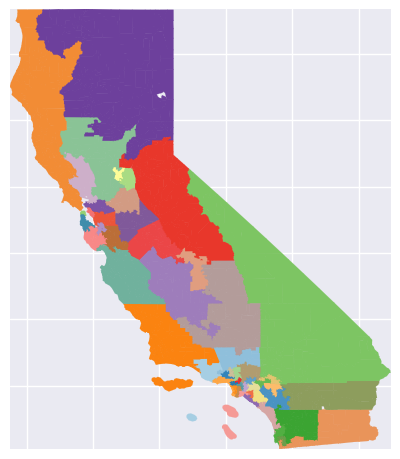
\includegraphics[width=5in,height=3in,keepaspectratio]{../maps/CA/static/before.png}
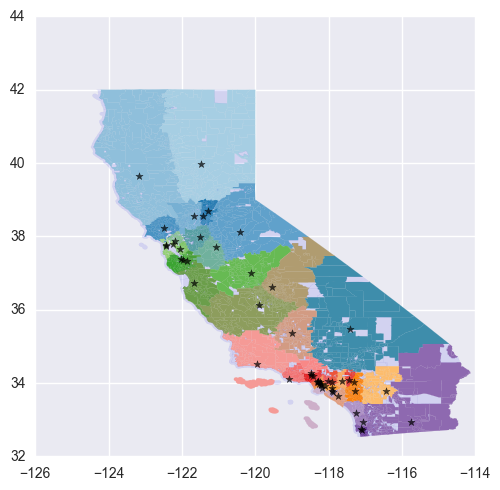
\includegraphics[width=5in,height=3in,keepaspectratio]{../maps/CA/static/0_0_after.png}
\caption{ New Districts ($\alpha_w$ = 1) }
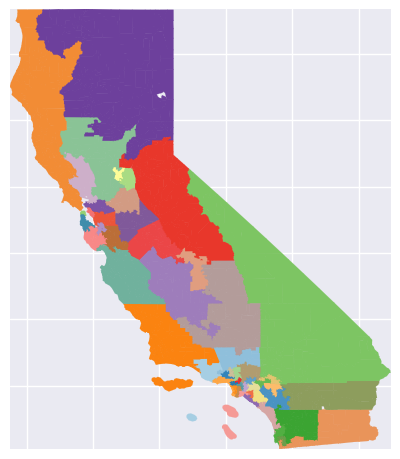
\includegraphics[width=5in,height=3in,keepaspectratio]{../maps/CA/static/before.png}
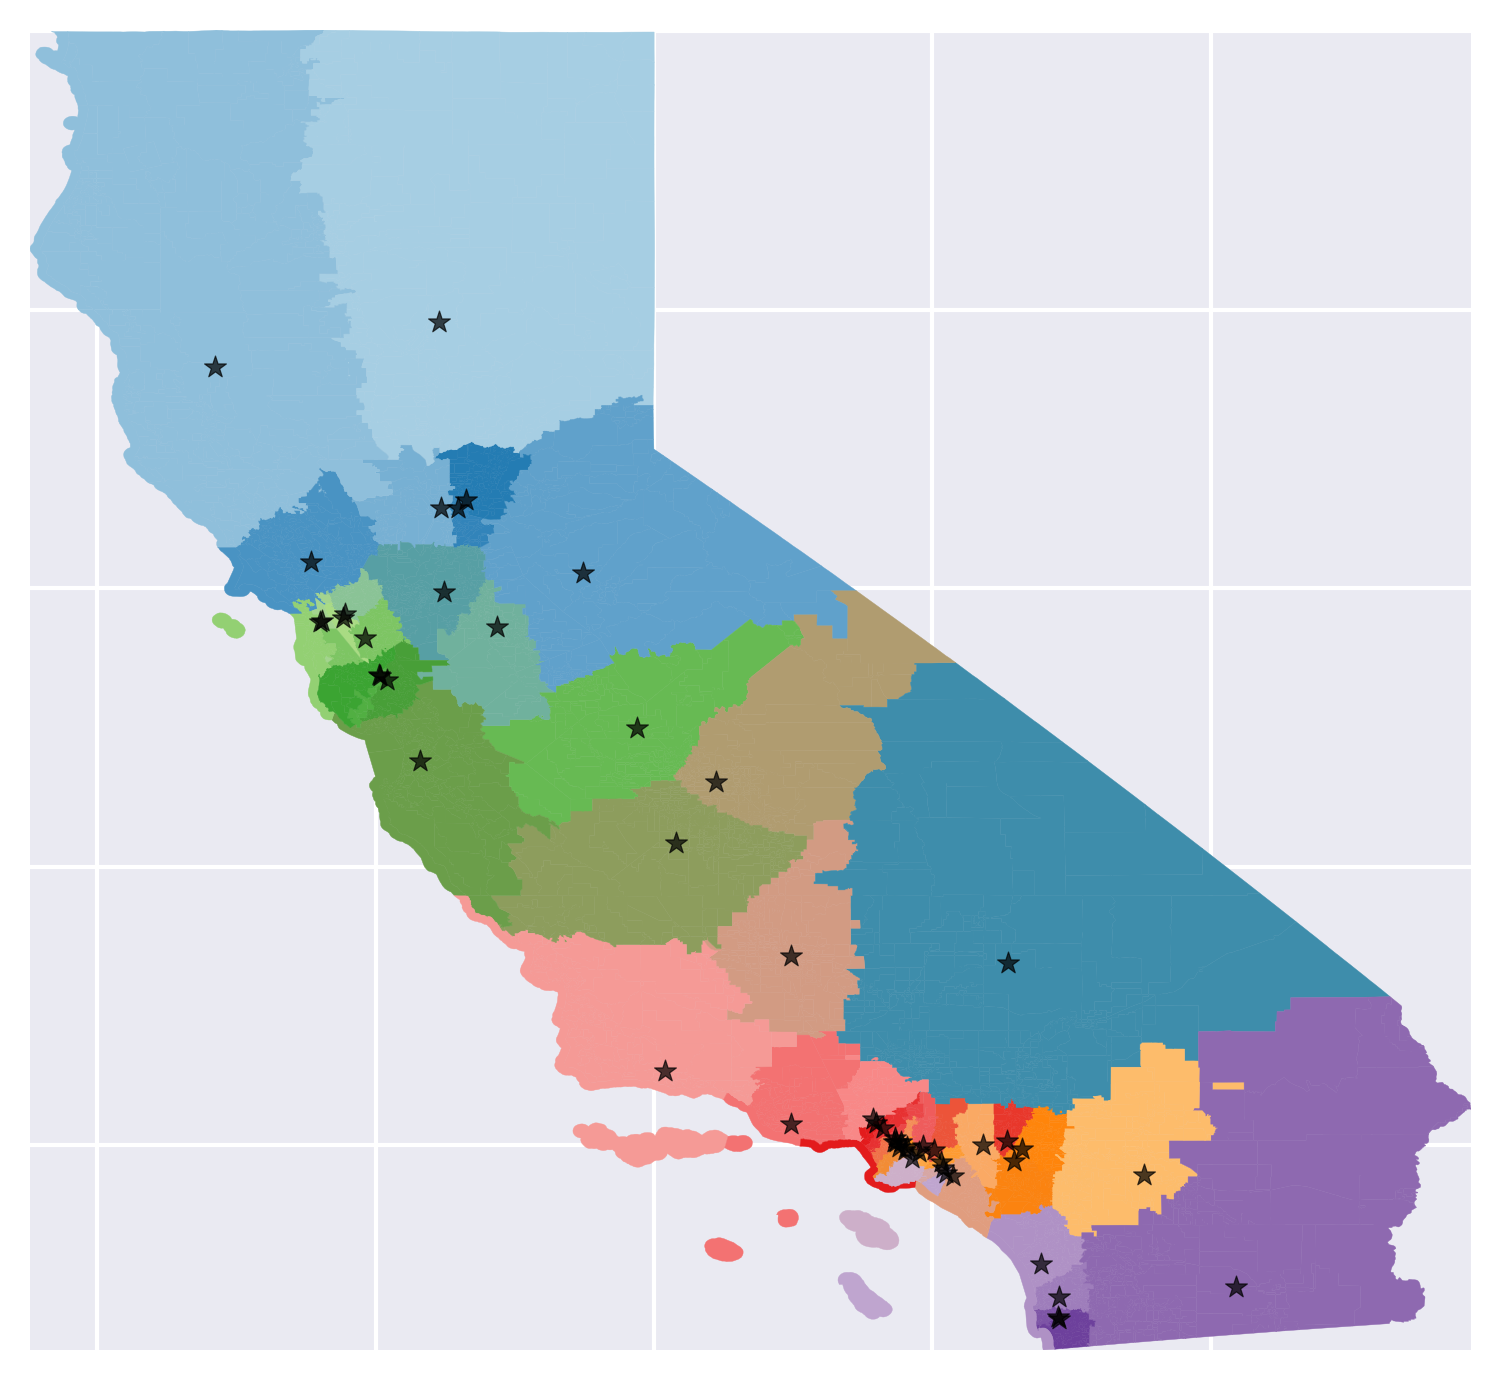
\includegraphics[width=5in,height=3in,keepaspectratio]{../maps/CA/static/0_25_after.png}
\end{figure}

\clearpage
\newpage

\begin{figure}[htb!] \centering
\caption{ Politics: democratic population (placeholder)}
\includegraphics[width=6in]{../analysis/CA/R_pct_kde.pdf}
\caption{ Demographics: black population }
\includegraphics[width=6in]{../analysis/CA/black_pct_kde.pdf}
\caption{ Demographics: hispanic population }
\includegraphics[width=6in]{../analysis/CA/hisp_pct_kde.pdf}
\end{figure}

\clearpage
\newpage

\begin{figure}[htb!] \centering
\caption{ Politics: democratic population (placeholder)}
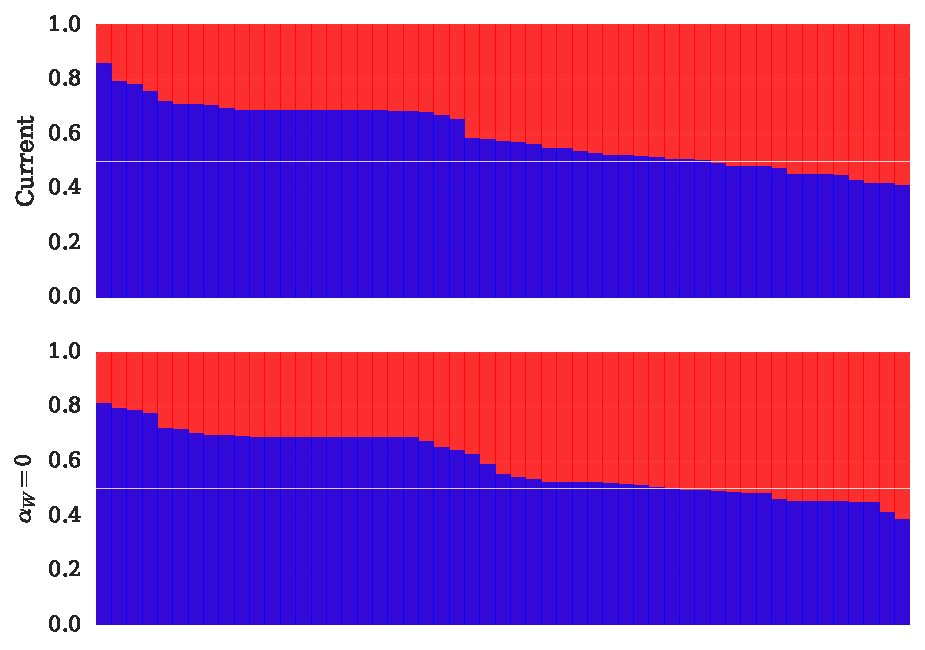
\includegraphics[width=6in]{../analysis/CA/barplot.pdf}
\end{figure}

\clearpage
\newpage

\subsection{Colorado}
\begin{figure}[htb!] \centering
\caption{ Current Districts }

\includegraphics[width=5in,height=3in,keepaspectratio]{../maps/CO/static/before.png}
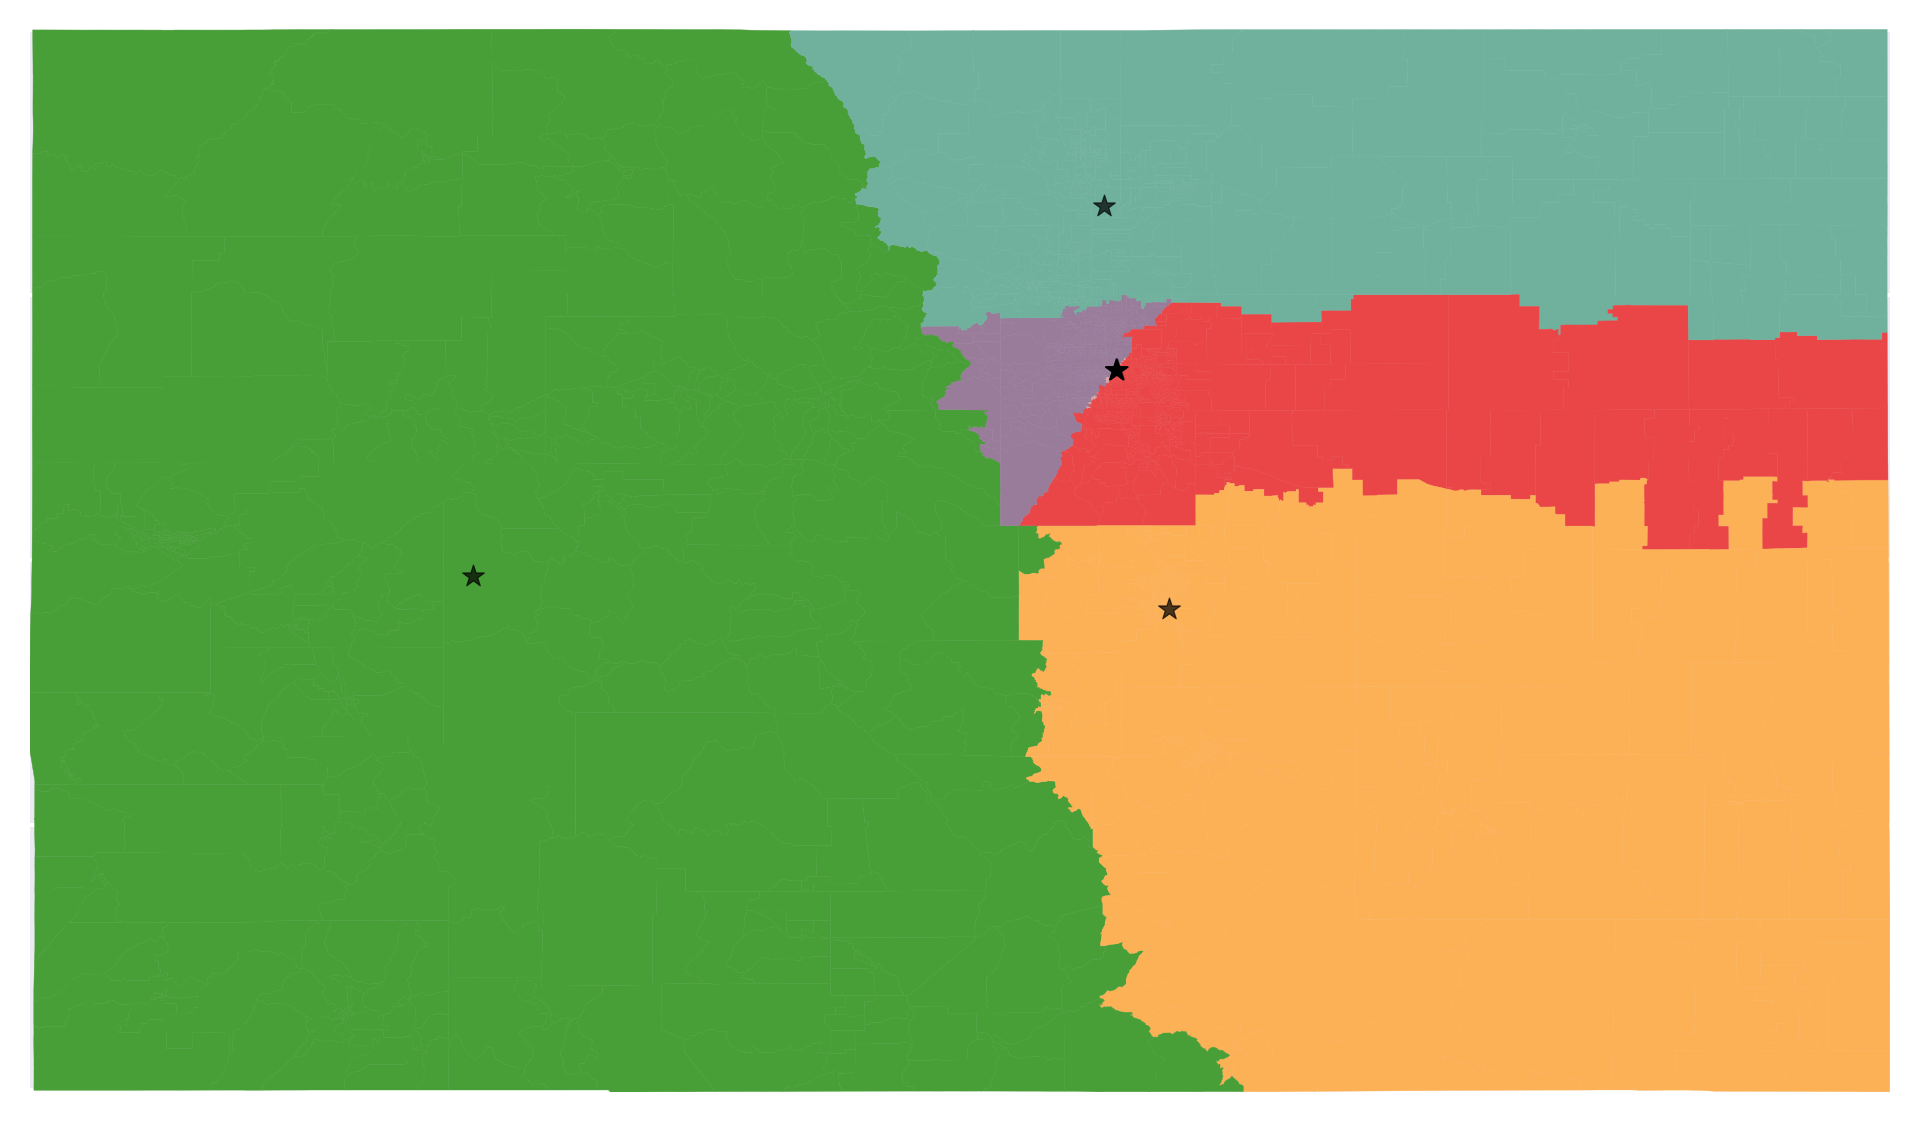
\includegraphics[width=5in,height=3in,keepaspectratio]{../maps/CO/static/0_0_after.png}
\caption{ New Districts ($\alpha_w$ = 1) }

\includegraphics[width=5in,height=3in,keepaspectratio]{../maps/CO/static/before.png}
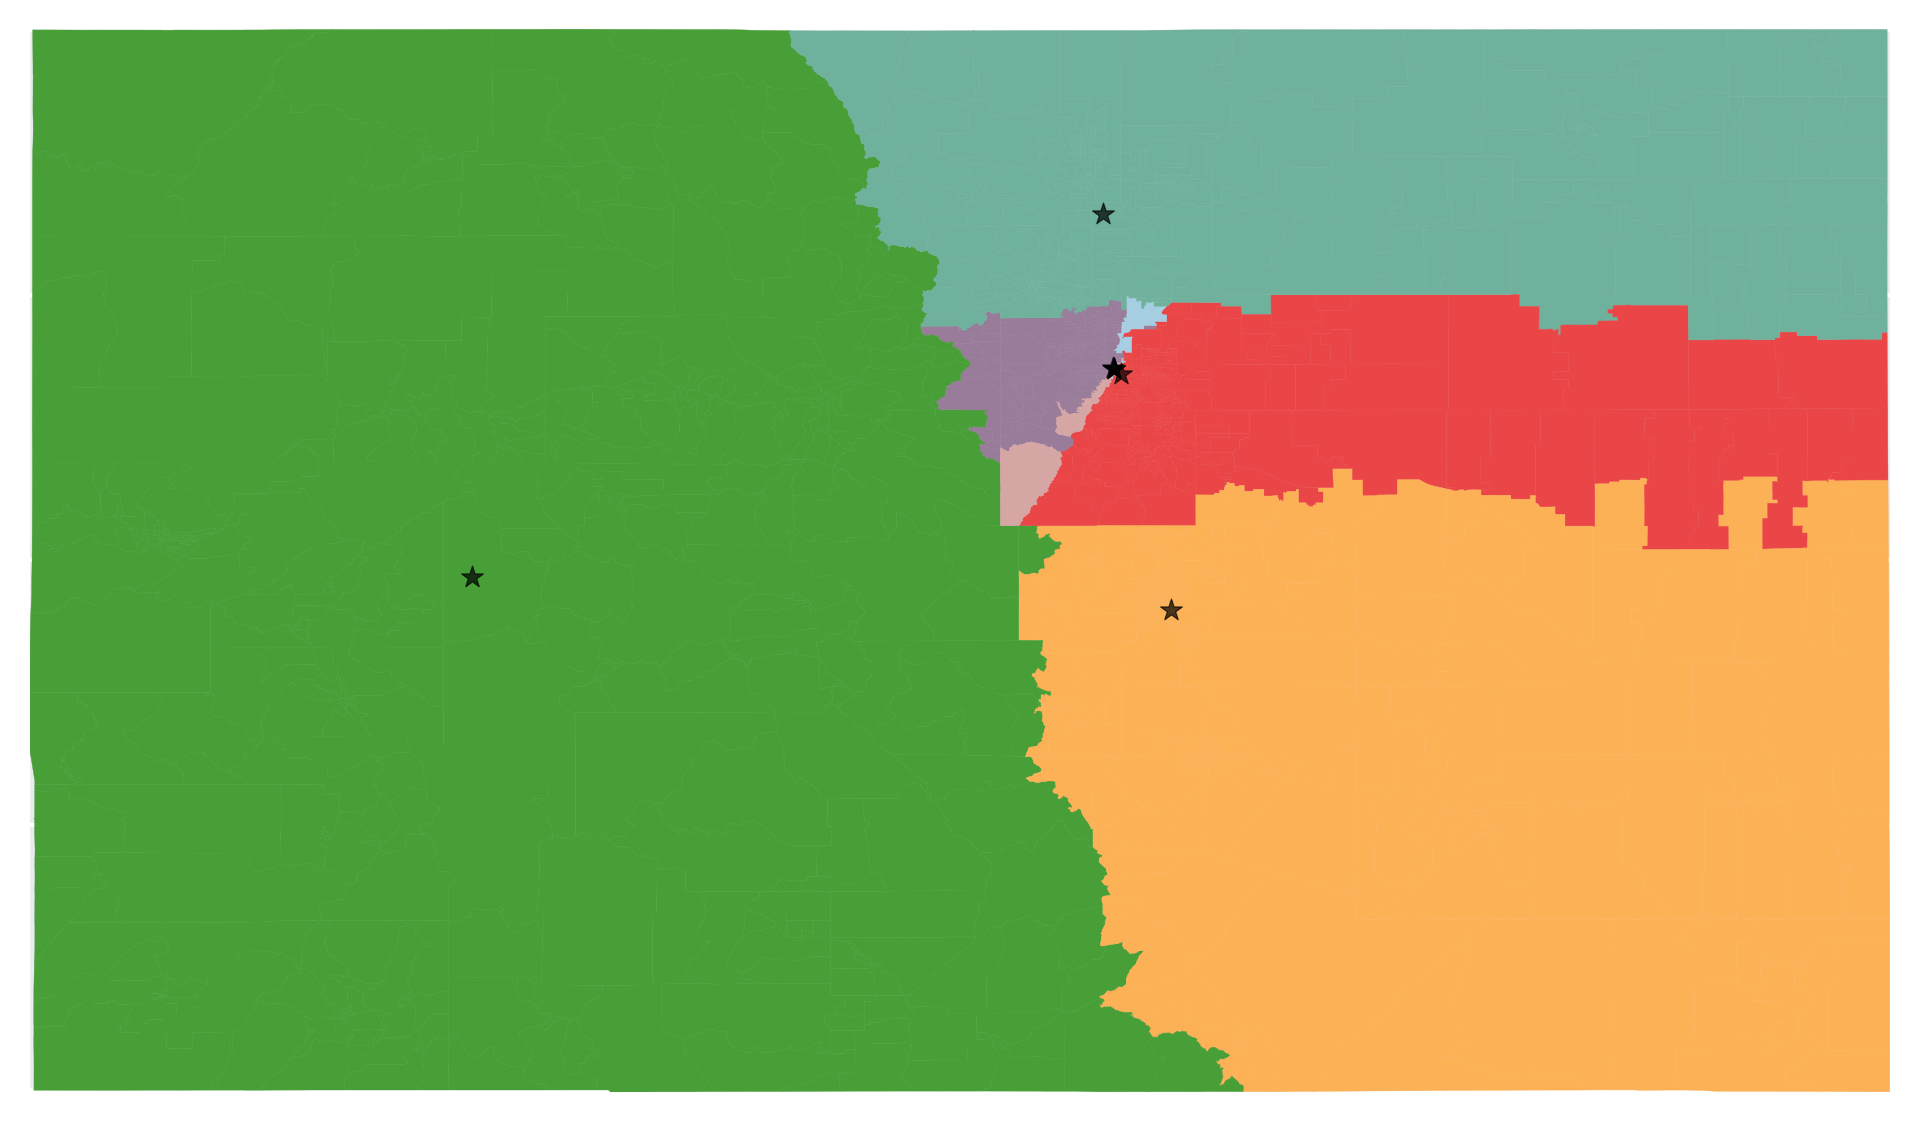
\includegraphics[width=5in,height=3in,keepaspectratio]{../maps/CO/static/0_25_after.png}
\end{figure}

\clearpage
\newpage

\begin{figure}[htb!] \centering
\caption{ Politics: democratic population (placeholder)}
\includegraphics[width=6in]{../analysis/CO/R_pct_kde.pdf}
\caption{ Demographics: black population }
\includegraphics[width=6in]{../analysis/CO/black_pct_kde.pdf}
\caption{ Demographics: hispanic population }
\includegraphics[width=6in]{../analysis/CO/hisp_pct_kde.pdf}
\end{figure}

\clearpage
\newpage

\begin{figure}[htb!] \centering
\caption{ Politics: democratic population (placeholder)}
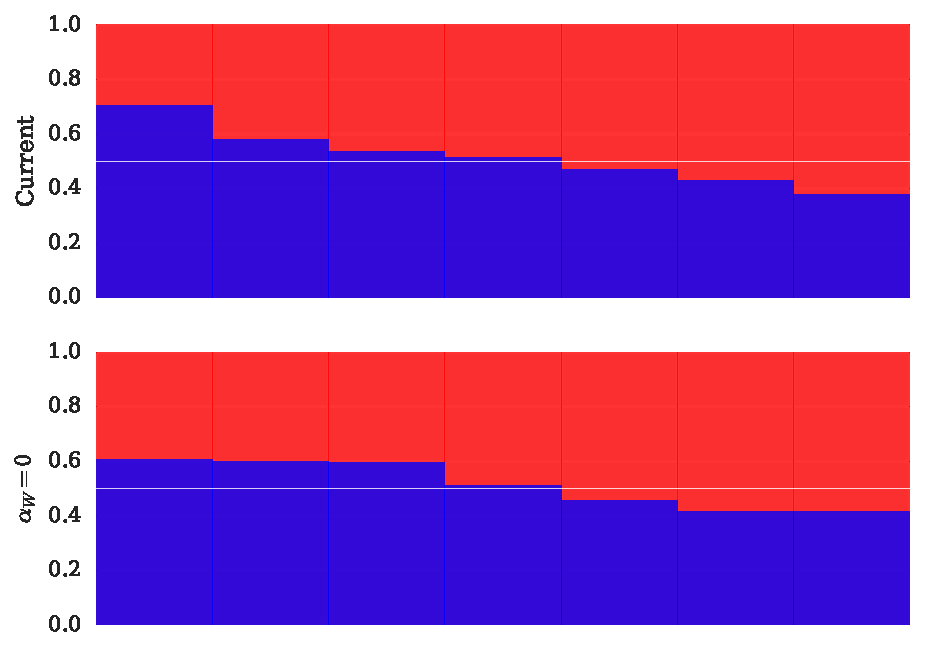
\includegraphics[width=6in]{../analysis/CO/barplot.pdf}
\end{figure}

\clearpage
\newpage

\subsection{Connecticut}
\begin{figure}[htb!] \centering
\caption{ Current Districts }
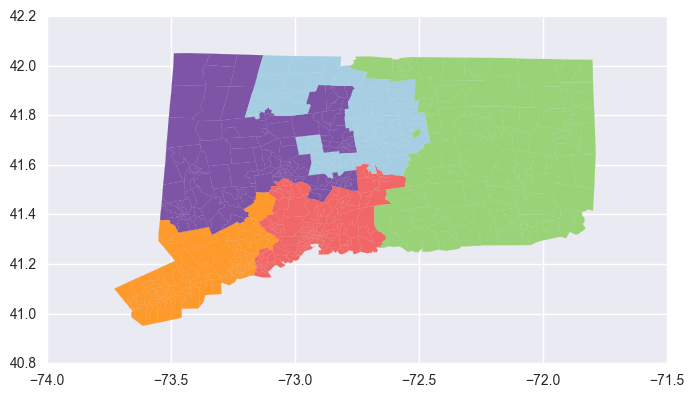
\includegraphics[width=4in,height=3in,keepaspectratio]{../maps/CT/static/before.png}
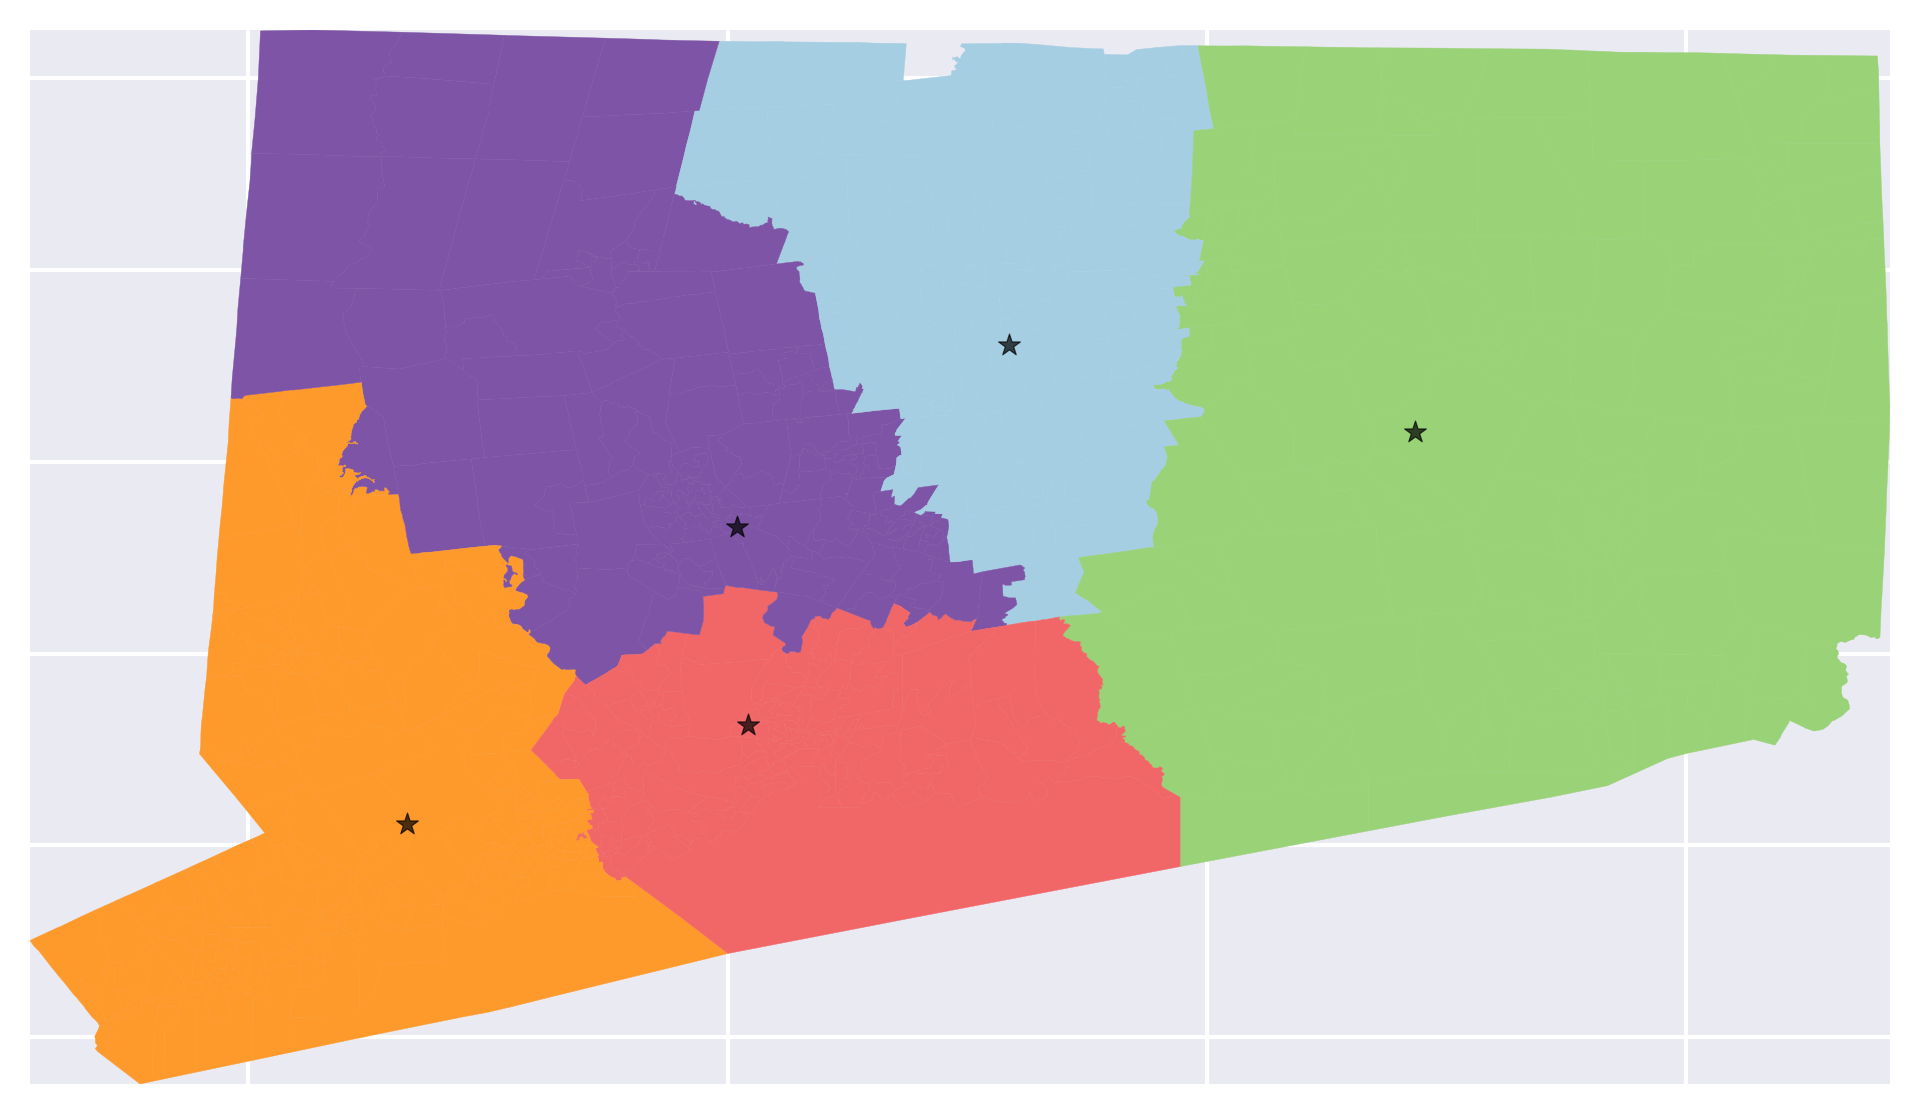
\includegraphics[width=4in,height=3in,keepaspectratio]{../maps/CT/static/0_0_after.png}
\caption{ New Districts ($\alpha_w$ = 1) }
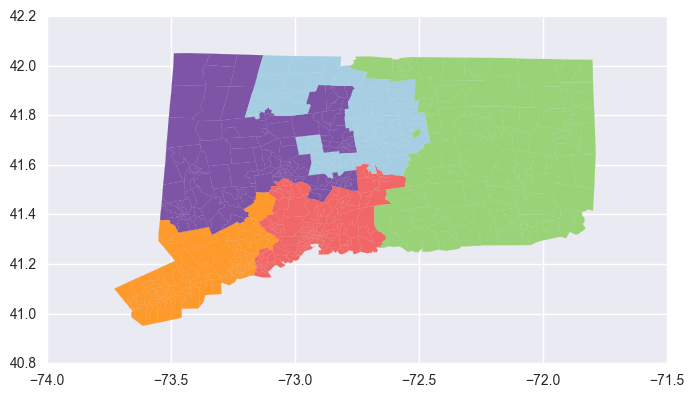
\includegraphics[width=4in,height=3in,keepaspectratio]{../maps/CT/static/before.png}
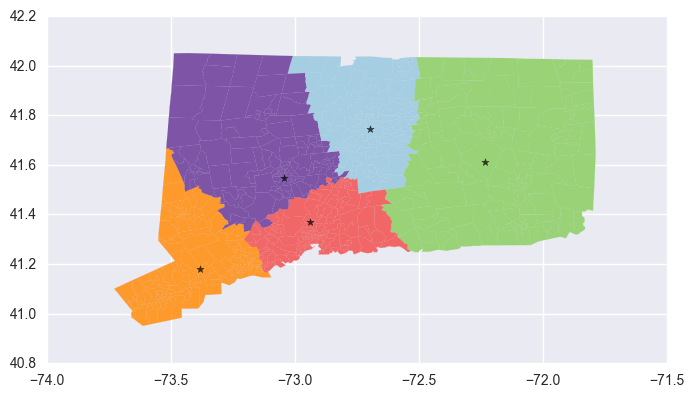
\includegraphics[width=4in,height=3in,keepaspectratio]{../maps/CT/static/0_25_after.png}
\end{figure}

\clearpage
\newpage

\begin{figure}[htb!] \centering
\caption{ Politics: democratic population (placeholder)}
\includegraphics[width=6in]{../analysis/CT/R_pct_kde.pdf}
\caption{ Demographics: black population }
\includegraphics[width=6in]{../analysis/CT/black_pct_kde.pdf}
\caption{ Demographics: hispanic population }
\includegraphics[width=6in]{../analysis/CT/hisp_pct_kde.pdf}
\end{figure}

\clearpage
\newpage

\begin{figure}[htb!] \centering
\caption{ Politics: democratic population (placeholder)}
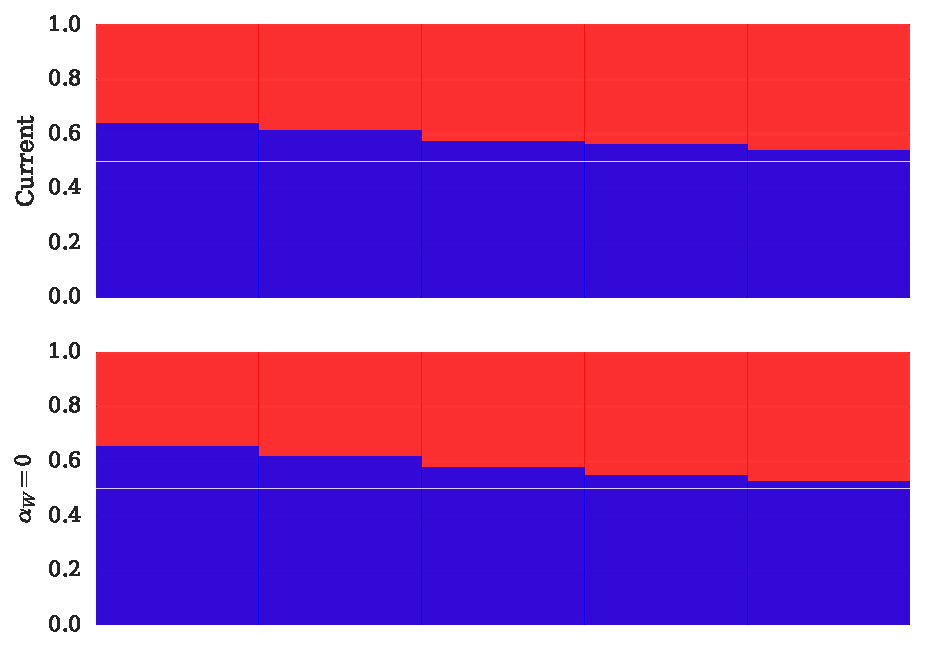
\includegraphics[width=6in]{../analysis/CT/barplot.pdf}
\end{figure}

\clearpage
\newpage

\subsection{Florida}
\begin{figure}[htb!] \centering
\caption{ Current Districts }
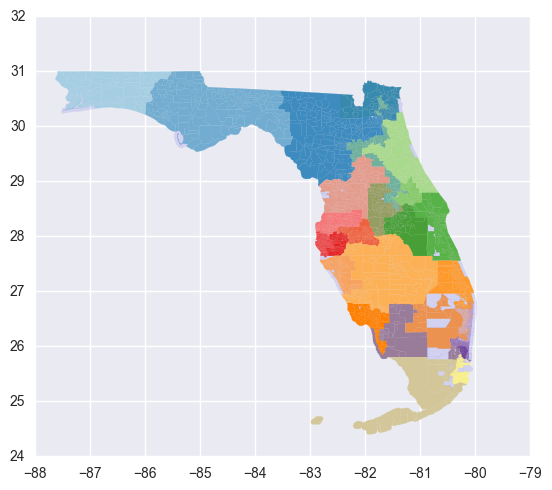
\includegraphics[width=5in,height=3in,keepaspectratio]{../maps/FL/static/before.png}
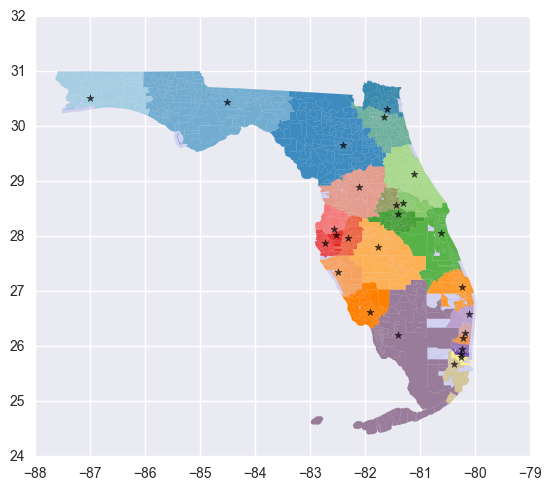
\includegraphics[width=5in,height=3in,keepaspectratio]{../maps/FL/static/0_0_after.png}
\caption{ New Districts ($\alpha_w$ = 1) }
\includegraphics[width=5in,height=3in,keepaspectratio]{../maps/FL/static/before.png}
\includegraphics[width=5in,height=3in,keepaspectratio]{../maps/FL/static/0_25_after.png}
\end{figure}

\clearpage
\newpage

\begin{figure}[htb!] \centering
\caption{ Politics: democratic population (placeholder)}
\includegraphics[width=6in]{../analysis/FL/R_pct_kde.pdf}
\caption{ Demographics: black population }
\includegraphics[width=6in]{../analysis/FL/black_pct_kde.pdf}
\caption{ Demographics: hispanic population }
\includegraphics[width=6in]{../analysis/FL/hisp_pct_kde.pdf}
\end{figure}

\clearpage
\newpage

\begin{figure}[htb!] \centering
\caption{ Politics: democratic population (placeholder)}
\includegraphics[width=6in]{../analysis/FL/barplot.pdf}
\end{figure}

\clearpage
\newpage

\subsection{Georgia}
\begin{figure}[htb!] \centering
\caption{ Current Districts }
\includegraphics[width=5in,height=3in,keepaspectratio]{../maps/GA/static/before.png}
\includegraphics[width=5in,height=3in,keepaspectratio]{../maps/GA/static/0_0_after.png}
\caption{ New Districts ($\alpha_w$ = 1) }
\includegraphics[width=5in,height=3in,keepaspectratio]{../maps/GA/static/before.png}
\includegraphics[width=5in,height=3in,keepaspectratio]{../maps/GA/static/0_25_after.png}
\end{figure}

\clearpage
\newpage

\begin{figure}[htb!] \centering
\caption{ Politics: democratic population (placeholder)}
\includegraphics[width=6in]{../analysis/GA/R_pct_kde.pdf}
\caption{ Demographics: black population }
\includegraphics[width=6in]{../analysis/GA/black_pct_kde.pdf}
\caption{ Demographics: hispanic population }
\includegraphics[width=6in]{../analysis/GA/hisp_pct_kde.pdf}
\end{figure}

\clearpage
\newpage

\begin{figure}[htb!] \centering
\caption{ Politics: democratic population (placeholder)}
\includegraphics[width=6in]{../analysis/GA/barplot.pdf}
\end{figure}

\clearpage
\newpage

\subsection{Hawaii}
\begin{figure}[htb!] \centering
\caption{ Current Districts }
\includegraphics[width=5in,height=3in,keepaspectratio]{../maps/HI/static/before.png}
\includegraphics[width=5in,height=3in,keepaspectratio]{../maps/HI/static/0_0_after.png}
\caption{ New Districts ($\alpha_w$ = 1) }
\includegraphics[width=5in,height=3in,keepaspectratio]{../maps/HI/static/before.png}
\includegraphics[width=5in,height=3in,keepaspectratio]{../maps/HI/static/0_25_after.png}
\end{figure}

\clearpage
\newpage

\begin{figure}[htb!] \centering
\caption{ Politics: democratic population (placeholder)}
\includegraphics[width=6in]{../analysis/HI/R_pct_kde.pdf}
\caption{ Demographics: black population }
\includegraphics[width=6in]{../analysis/HI/black_pct_kde.pdf}
\caption{ Demographics: hispanic population }
\includegraphics[width=6in]{../analysis/HI/hisp_pct_kde.pdf}
\end{figure}

\clearpage
\newpage

\begin{figure}[htb!] \centering
\caption{ Politics: democratic population (placeholder)}
\includegraphics[width=6in]{../analysis/HI/barplot.pdf}
\end{figure}

\clearpage
\newpage

\subsection{Iowa}
\begin{figure}[htb!] \centering
\caption{ Current Districts }
\includegraphics[width=4in,height=3in,keepaspectratio]{../maps/IA/static/before.png}
\includegraphics[width=4in,height=3in,keepaspectratio]{../maps/IA/static/0_0_after.png}
\caption{ New Districts ($\alpha_w$ = 1) }
\includegraphics[width=4in,height=3in,keepaspectratio]{../maps/IA/static/before.png}
\includegraphics[width=4in,height=3in,keepaspectratio]{../maps/IA/static/0_25_after.png}
\end{figure}

\clearpage
\newpage

\begin{figure}[htb!] \centering
\caption{ Politics: democratic population (placeholder)}
\includegraphics[width=6in]{../analysis/IA/R_pct_kde.pdf}
\caption{ Demographics: black population }
\includegraphics[width=6in]{../analysis/IA/black_pct_kde.pdf}
\caption{ Demographics: hispanic population }
\includegraphics[width=6in]{../analysis/IA/hisp_pct_kde.pdf}
\end{figure}

\clearpage
\newpage

\begin{figure}[htb!] \centering
\caption{ Politics: democratic population (placeholder)}
\includegraphics[width=6in]{../analysis/IA/barplot.pdf}
\end{figure}

\clearpage
\newpage

\subsection{Idaho}
\begin{figure}[htb!] \centering
\caption{ Current Districts }
\includegraphics[width=5in,height=3in,keepaspectratio]{../maps/ID/static/before.png}
\includegraphics[width=5in,height=3in,keepaspectratio]{../maps/ID/static/0_0_after.png}
\caption{ New Districts ($\alpha_w$ = 1) }
\includegraphics[width=5in,height=3in,keepaspectratio]{../maps/ID/static/before.png}
\includegraphics[width=5in,height=3in,keepaspectratio]{../maps/ID/static/0_25_after.png}
\end{figure}

\clearpage
\newpage

\begin{figure}[htb!] \centering
\caption{ Politics: democratic population (placeholder)}
\includegraphics[width=6in]{../analysis/ID/R_pct_kde.pdf}
\caption{ Demographics: black population }
\includegraphics[width=6in]{../analysis/ID/black_pct_kde.pdf}
\caption{ Demographics: hispanic population }
\includegraphics[width=6in]{../analysis/ID/hisp_pct_kde.pdf}
\end{figure}

\clearpage
\newpage

\begin{figure}[htb!] \centering
\caption{ Politics: democratic population (placeholder)}
\includegraphics[width=6in]{../analysis/ID/barplot.pdf}
\end{figure}

\clearpage
\newpage

\subsection{Illinois}
\begin{figure}[htb!] \centering
\caption{ Current Districts }
\includegraphics[width=5in,height=3in,keepaspectratio]{../maps/IL/static/before.png}
\includegraphics[width=5in,height=3in,keepaspectratio]{../maps/IL/static/0_0_after.png}
\caption{ New Districts ($\alpha_w$ = 1) }
\includegraphics[width=5in,height=3in,keepaspectratio]{../maps/IL/static/before.png}
\includegraphics[width=5in,height=3in,keepaspectratio]{../maps/IL/static/0_25_after.png}
\end{figure}

\clearpage
\newpage

\begin{figure}[htb!] \centering
\caption{ Politics: democratic population (placeholder)}
\includegraphics[width=6in]{../analysis/IL/R_pct_kde.pdf}
\caption{ Demographics: black population }
\includegraphics[width=6in]{../analysis/IL/black_pct_kde.pdf}
\caption{ Demographics: hispanic population }
\includegraphics[width=6in]{../analysis/IL/hisp_pct_kde.pdf}
\end{figure}

\clearpage
\newpage

\begin{figure}[htb!] \centering
\caption{ Politics: democratic population (placeholder)}
\includegraphics[width=6in]{../analysis/IL/barplot.pdf}
\end{figure}

\clearpage
\newpage

\subsection{Indiana}
\begin{figure}[htb!] \centering
\caption{ Current Districts }
\includegraphics[width=5in,height=3in,keepaspectratio]{../maps/IN/static/before.png}
\includegraphics[width=5in,height=3in,keepaspectratio]{../maps/IN/static/0_0_after.png}
\caption{ New Districts ($\alpha_w$ = 1) }
\includegraphics[width=5in,height=3in,keepaspectratio]{../maps/IN/static/before.png}
\includegraphics[width=5in,height=3in,keepaspectratio]{../maps/IN/static/0_25_after.png}
\end{figure}

\clearpage
\newpage

\begin{figure}[htb!] \centering
\caption{ Politics: democratic population (placeholder)}
\includegraphics[width=6in]{../analysis/IN/R_pct_kde.pdf}
\caption{ Demographics: black population }
\includegraphics[width=6in]{../analysis/IN/black_pct_kde.pdf}
\caption{ Demographics: hispanic population }
\includegraphics[width=6in]{../analysis/IN/hisp_pct_kde.pdf}
\end{figure}

\clearpage
\newpage

\begin{figure}[htb!] \centering
\caption{ Politics: democratic population (placeholder)}
\includegraphics[width=6in]{../analysis/IN/barplot.pdf}
\end{figure}

\clearpage
\newpage

\subsection{Kansas}
\begin{figure}[htb!] \centering
\caption{ Current Districts }
\includegraphics[width=4in,height=3in,keepaspectratio]{../maps/KS/static/before.png}
\includegraphics[width=4in,height=3in,keepaspectratio]{../maps/KS/static/0_0_after.png}
\caption{ New Districts ($\alpha_w$ = 1) }
\includegraphics[width=4in,height=3in,keepaspectratio]{../maps/KS/static/before.png}
\includegraphics[width=4in,height=3in,keepaspectratio]{../maps/KS/static/0_25_after.png}
\end{figure}

\clearpage
\newpage

\begin{figure}[htb!] \centering
\caption{ Politics: democratic population (placeholder)}
\includegraphics[width=6in]{../analysis/KS/R_pct_kde.pdf}
\caption{ Demographics: black population }
\includegraphics[width=6in]{../analysis/KS/black_pct_kde.pdf}
\caption{ Demographics: hispanic population }
\includegraphics[width=6in]{../analysis/KS/hisp_pct_kde.pdf}
\end{figure}

\clearpage
\newpage

\begin{figure}[htb!] \centering
\caption{ Politics: democratic population (placeholder)}
\includegraphics[width=6in]{../analysis/KS/barplot.pdf}
\end{figure}

\clearpage
\newpage

\subsection{Louisiana}
\begin{figure}[htb!] \centering
\caption{ Current Districts }
\includegraphics[width=5in,height=3in,keepaspectratio]{../maps/LA/static/before.png}
\includegraphics[width=5in,height=3in,keepaspectratio]{../maps/LA/static/0_0_after.png}
\caption{ New Districts ($\alpha_w$ = 1) }
\includegraphics[width=5in,height=3in,keepaspectratio]{../maps/LA/static/before.png}
\includegraphics[width=5in,height=3in,keepaspectratio]{../maps/LA/static/0_25_after.png}
\end{figure}

\clearpage
\newpage

\begin{figure}[htb!] \centering
\caption{ Politics: democratic population (placeholder)}
\includegraphics[width=6in]{../analysis/LA/R_pct_kde.pdf}
\caption{ Demographics: black population }
\includegraphics[width=6in]{../analysis/LA/black_pct_kde.pdf}
\caption{ Demographics: hispanic population }
\includegraphics[width=6in]{../analysis/LA/hisp_pct_kde.pdf}
\end{figure}

\clearpage
\newpage

\begin{figure}[htb!] \centering
\caption{ Politics: democratic population (placeholder)}
\includegraphics[width=6in]{../analysis/LA/barplot.pdf}
\end{figure}

\clearpage
\newpage

\subsection{Massachusetts}
\begin{figure}[htb!] \centering
\caption{ Current Districts }
\includegraphics[width=5in,height=3in,keepaspectratio]{../maps/MA/static/before.png}
\includegraphics[width=5in,height=3in,keepaspectratio]{../maps/MA/static/0_0_after.png}
\caption{ New Districts ($\alpha_w$ = 1) }
\includegraphics[width=5in,height=3in,keepaspectratio]{../maps/MA/static/before.png}
\includegraphics[width=5in,height=3in,keepaspectratio]{../maps/MA/static/0_25_after.png}
\end{figure}

\clearpage
\newpage

\begin{figure}[htb!] \centering
\caption{ Politics: democratic population (placeholder)}
\includegraphics[width=6in]{../analysis/MA/R_pct_kde.pdf}
\caption{ Demographics: black population }
\includegraphics[width=6in]{../analysis/MA/black_pct_kde.pdf}
\caption{ Demographics: hispanic population }
\includegraphics[width=6in]{../analysis/MA/hisp_pct_kde.pdf}
\end{figure}

\clearpage
\newpage

\begin{figure}[htb!] \centering
\caption{ Politics: democratic population (placeholder)}
\includegraphics[width=6in]{../analysis/MA/barplot.pdf}
\end{figure}

\clearpage
\newpage

\subsection{Maryland}
\begin{figure}[htb!] \centering
\caption{ Current Districts }
\includegraphics[width=5in,height=3in,keepaspectratio]{../maps/MD/static/before.png}
\includegraphics[width=5in,height=3in,keepaspectratio]{../maps/MD/static/0_0_after.png}
\caption{ New Districts ($\alpha_w$ = 1) }
\includegraphics[width=5in,height=3in,keepaspectratio]{../maps/MD/static/before.png}
\includegraphics[width=5in,height=3in,keepaspectratio]{../maps/MD/static/0_25_after.png}
\end{figure}

\clearpage
\newpage

\begin{figure}[htb!] \centering
\caption{ Politics: democratic population (placeholder)}
\includegraphics[width=6in]{../analysis/MD/R_pct_kde.pdf}
\caption{ Demographics: black population }
\includegraphics[width=6in]{../analysis/MD/black_pct_kde.pdf}
\caption{ Demographics: hispanic population }
\includegraphics[width=6in]{../analysis/MD/hisp_pct_kde.pdf}
\end{figure}

\clearpage
\newpage

\begin{figure}[htb!] \centering
\caption{ Politics: democratic population (placeholder)}
\includegraphics[width=6in]{../analysis/MD/barplot.pdf}
\end{figure}

\clearpage
\newpage

\subsection{Michigan}
\begin{figure}[htb!] \centering
\caption{ Current Districts }
\includegraphics[width=5in,height=3in,keepaspectratio]{../maps/MI/static/before.png}
\includegraphics[width=5in,height=3in,keepaspectratio]{../maps/MI/static/0_0_after.png}
\caption{ New Districts ($\alpha_w$ = 1) }
\includegraphics[width=5in,height=3in,keepaspectratio]{../maps/MI/static/before.png}
\includegraphics[width=5in,height=3in,keepaspectratio]{../maps/MI/static/0_25_after.png}
\end{figure}

\clearpage
\newpage

\begin{figure}[htb!] \centering
\caption{ Politics: democratic population (placeholder)}
\includegraphics[width=6in]{../analysis/MI/R_pct_kde.pdf}
\caption{ Demographics: black population }
\includegraphics[width=6in]{../analysis/MI/black_pct_kde.pdf}
\caption{ Demographics: hispanic population }
\includegraphics[width=6in]{../analysis/MI/hisp_pct_kde.pdf}
\end{figure}

\clearpage
\newpage

\begin{figure}[htb!] \centering
\caption{ Politics: democratic population (placeholder)}
\includegraphics[width=6in]{../analysis/MI/barplot.pdf}
\end{figure}

\clearpage
\newpage

\subsection{Minnesota}
\begin{figure}[htb!] \centering
\caption{ Current Districts }
\includegraphics[width=5in,height=3in,keepaspectratio]{../maps/MN/static/before.png}
\includegraphics[width=5in,height=3in,keepaspectratio]{../maps/MN/static/0_0_after.png}
\caption{ New Districts ($\alpha_w$ = 1) }
\includegraphics[width=5in,height=3in,keepaspectratio]{../maps/MN/static/before.png}
\includegraphics[width=5in,height=3in,keepaspectratio]{../maps/MN/static/0_25_after.png}
\end{figure}

\clearpage
\newpage

\begin{figure}[htb!] \centering
\caption{ Politics: democratic population (placeholder)}
\includegraphics[width=6in]{../analysis/MN/R_pct_kde.pdf}
\caption{ Demographics: black population }
\includegraphics[width=6in]{../analysis/MN/black_pct_kde.pdf}
\caption{ Demographics: hispanic population }
\includegraphics[width=6in]{../analysis/MN/hisp_pct_kde.pdf}
\end{figure}

\clearpage
\newpage

\begin{figure}[htb!] \centering
\caption{ Politics: democratic population (placeholder)}
\includegraphics[width=6in]{../analysis/MN/barplot.pdf}
\end{figure}

\clearpage
\newpage

\subsection{Missouri}
\begin{figure}[htb!] \centering
\caption{ Current Districts }
\includegraphics[width=5in,height=3in,keepaspectratio]{../maps/MO/static/before.png}
\includegraphics[width=5in,height=3in,keepaspectratio]{../maps/MO/static/0_0_after.png}
\caption{ New Districts ($\alpha_w$ = 1) }
\includegraphics[width=5in,height=3in,keepaspectratio]{../maps/MO/static/before.png}
\includegraphics[width=5in,height=3in,keepaspectratio]{../maps/MO/static/0_25_after.png}
\end{figure}

\clearpage
\newpage

\begin{figure}[htb!] \centering
\caption{ Politics: democratic population (placeholder)}
\includegraphics[width=6in]{../analysis/MO/R_pct_kde.pdf}
\caption{ Demographics: black population }
\includegraphics[width=6in]{../analysis/MO/black_pct_kde.pdf}
\caption{ Demographics: hispanic population }
\includegraphics[width=6in]{../analysis/MO/hisp_pct_kde.pdf}
\end{figure}

\clearpage
\newpage

\begin{figure}[htb!] \centering
\caption{ Politics: democratic population (placeholder)}
\includegraphics[width=6in]{../analysis/MO/barplot.pdf}
\end{figure}

\clearpage
\newpage

\subsection{Mississippi}
\begin{figure}[htb!] \centering
\caption{ Current Districts }
\includegraphics[width=5in,height=3in,keepaspectratio]{../maps/MS/static/before.png}
\includegraphics[width=5in,height=3in,keepaspectratio]{../maps/MS/static/0_0_after.png}
\caption{ New Districts ($\alpha_w$ = 1) }
\includegraphics[width=5in,height=3in,keepaspectratio]{../maps/MS/static/before.png}
\includegraphics[width=5in,height=3in,keepaspectratio]{../maps/MS/static/0_25_after.png}
\end{figure}

\clearpage
\newpage

\begin{figure}[htb!] \centering
\caption{ Politics: democratic population (placeholder)}
\includegraphics[width=6in]{../analysis/MS/R_pct_kde.pdf}
\caption{ Demographics: black population }
\includegraphics[width=6in]{../analysis/MS/black_pct_kde.pdf}
\caption{ Demographics: hispanic population }
\includegraphics[width=6in]{../analysis/MS/hisp_pct_kde.pdf}
\end{figure}

\clearpage
\newpage

\begin{figure}[htb!] \centering
\caption{ Politics: democratic population (placeholder)}
\includegraphics[width=6in]{../analysis/MS/barplot.pdf}
\end{figure}

\clearpage
\newpage

\subsection{North Carolina}
\begin{figure}[htb!] \centering
\caption{ Current Districts }
\includegraphics[width=5in,height=3in,keepaspectratio]{../maps/NC/static/before.png}
\includegraphics[width=5in,height=3in,keepaspectratio]{../maps/NC/static/0_0_after.png}
\caption{ New Districts ($\alpha_w$ = 1) }
\includegraphics[width=5in,height=3in,keepaspectratio]{../maps/NC/static/before.png}
\includegraphics[width=5in,height=3in,keepaspectratio]{../maps/NC/static/0_25_after.png}
\end{figure}

\clearpage
\newpage

\begin{figure}[htb!] \centering
\caption{ Politics: democratic population (placeholder)}
\includegraphics[width=6in]{../analysis/NC/R_pct_kde.pdf}
\caption{ Demographics: black population }
\includegraphics[width=6in]{../analysis/NC/black_pct_kde.pdf}
\caption{ Demographics: hispanic population }
\includegraphics[width=6in]{../analysis/NC/hisp_pct_kde.pdf}
\end{figure}

\clearpage
\newpage

\begin{figure}[htb!] \centering
\caption{ Politics: democratic population (placeholder)}
\includegraphics[width=6in]{../analysis/NC/barplot.pdf}
\end{figure}

\clearpage
\newpage

\subsection{New Jersey}
\begin{figure}[htb!] \centering
\caption{ Current Districts }
\includegraphics[width=5in,height=3in,keepaspectratio]{../maps/NJ/static/before.png}
\includegraphics[width=5in,height=3in,keepaspectratio]{../maps/NJ/static/0_0_after.png}
\caption{ New Districts ($\alpha_w$ = 1) }
\includegraphics[width=5in,height=3in,keepaspectratio]{../maps/NJ/static/before.png}
\includegraphics[width=5in,height=3in,keepaspectratio]{../maps/NJ/static/0_25_after.png}
\end{figure}

\clearpage
\newpage

\begin{figure}[htb!] \centering
\caption{ Politics: democratic population (placeholder)}
\includegraphics[width=6in]{../analysis/NJ/R_pct_kde.pdf}
\caption{ Demographics: black population }
\includegraphics[width=6in]{../analysis/NJ/black_pct_kde.pdf}
\caption{ Demographics: hispanic population }
\includegraphics[width=6in]{../analysis/NJ/hisp_pct_kde.pdf}
\end{figure}

\clearpage
\newpage

\begin{figure}[htb!] \centering
\caption{ Politics: democratic population (placeholder)}
\includegraphics[width=6in]{../analysis/NJ/barplot.pdf}
\end{figure}

\clearpage
\newpage

\subsection{New Mexico}
\begin{figure}[htb!] \centering
\caption{ Current Districts }
\includegraphics[width=5in,height=3in,keepaspectratio]{../maps/NM/static/before.png}
\includegraphics[width=5in,height=3in,keepaspectratio]{../maps/NM/static/0_0_after.png}
\caption{ New Districts ($\alpha_w$ = 1) }
\includegraphics[width=5in,height=3in,keepaspectratio]{../maps/NM/static/before.png}
\includegraphics[width=5in,height=3in,keepaspectratio]{../maps/NM/static/0_25_after.png}
\end{figure}

\clearpage
\newpage

\begin{figure}[htb!] \centering
\caption{ Politics: democratic population (placeholder)}
\includegraphics[width=6in]{../analysis/NM/R_pct_kde.pdf}
\caption{ Demographics: black population }
\includegraphics[width=6in]{../analysis/NM/black_pct_kde.pdf}
\caption{ Demographics: hispanic population }
\includegraphics[width=6in]{../analysis/NM/hisp_pct_kde.pdf}
\end{figure}

\clearpage
\newpage

\begin{figure}[htb!] \centering
\caption{ Politics: democratic population (placeholder)}
\includegraphics[width=6in]{../analysis/NM/barplot.pdf}
\end{figure}

\clearpage
\newpage








\end{document}
